%\textsf{Usage scenarios.}

Figure~\ref{fig-wot-scenario} presents a typical WoT deployment scenario. 
A WoT Thing device together with a WoT Servient are placed inside the local network behind a forwarding proxy. 
A WoT Client that is located outside of this boundary wants to perform operations exposed via Thing description, uploaded by the WoT Thing and WoT Servient to a Things Directory located on a remote cloud or service. 
In order to do this it first needs to issue a discovery query to the Things Directory about relevant TD, which is usually done using semantic search capabilities. 
Next upon obtaining it, the WoT Client needs to make sure it has all relevant credentials that are needed to authenticate to the Forwarding proxy (if secure authentication on proxy is enabled), the WoT Servient and in some cases even to the end WoT Thing.
All required information about these potentially different credentials should be provided in the obtained Thing Description.  

\begin{figure*}[!t]
\centering
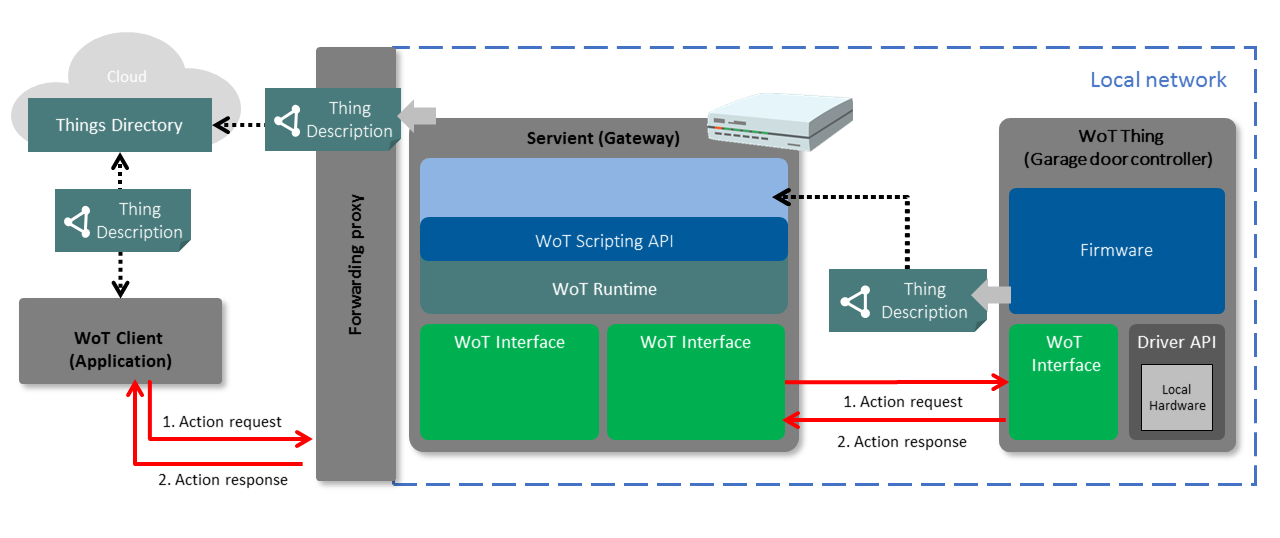
\includegraphics[width=6in]{figures/wot-scenario.png}
\caption{A Typical WoT deployment scenario}
\label{fig-wot-scenario}
\end{figure*}

